%% Nothing to modify here.
%% make sure to include this before anything else

\documentclass[10pt]{beamer}
\usetheme{Szeged}
\usenavigationsymbolstemplate{}
\usepackage{tgcursor}

% packages
\usepackage{color}
\usepackage{listings}

% color definitions
\definecolor{mygreen}{rgb}{0,0.6,0}
\definecolor{mygray}{rgb}{0.5,0.5,0.5}
\definecolor{mymauve}{rgb}{0.58,0,0.82}

% re-format the title frame page
\makeatletter
\def\supertitle#1{\gdef\@supertitle{#1}}%
\setbeamertemplate{title page}
{
  \vbox{}
  \vfill
  \begin{centering}
  \begin{beamercolorbox}[sep=8pt,center]{title}
      \usebeamerfont{supertitle}\@supertitle
   \end{beamercolorbox}
    \begin{beamercolorbox}[sep=8pt,center]{title}
      \usebeamerfont{title}\inserttitle\par%
      \ifx\insertsubtitle\@empty%
      \else%
        \vskip0.25em%
        {\usebeamerfont{subtitle}\usebeamercolor[fg]{subtitle}\insertsubtitle\par}%
      \fi%     
    \end{beamercolorbox}%
    \vskip1em\par
    \begin{beamercolorbox}[sep=8pt,center]{author}
      \usebeamerfont{author}\insertauthor
    \end{beamercolorbox}
    \begin{beamercolorbox}[sep=8pt,center]{institute}
      \usebeamerfont{institute}\insertinstitute
    \end{beamercolorbox}
    \begin{beamercolorbox}[sep=8pt,center]{date}
      \usebeamerfont{date}\insertdate
    \end{beamercolorbox}\vskip0.5em
    {\usebeamercolor[fg]{titlegraphic}\inserttitlegraphic\par}
  \end{centering}
  \vfill
}
\makeatother

% insert frame number
\expandafter\def\expandafter\insertshorttitle\expandafter{%
      \insertshorttitle\hfill%
\insertframenumber\,/\,\inserttotalframenumber}

% preset-listing options
\lstset{
  backgroundcolor=\color{white},   
  % choose the background color; 
  % you must add \usepackage{color} or \usepackage{xcolor}
  basicstyle=\footnotesize,
  % the size of the fonts that are used for the code
  breakatwhitespace=false,         
  % sets if automatic breaks should only happen at whitespace
  breaklines=true,                 % sets automatic line breaking
  captionpos=b,                    % sets the caption-position to bottom
  commentstyle=\color{mygreen},    % comment style
  % deletekeywords={...},            
  % if you want to delete keywords from the given language
  extendedchars=true,              
  % lets you use non-ASCII characters; 
  % for 8-bits encodings only, does not work with UTF-8
  frame=single,                    % adds a frame around the code
  keepspaces=true,                 
  % keeps spaces in text, 
  % useful for keeping indentation of code 
  % (possibly needs columns=flexible)
  keywordstyle=\color{blue},       % keyword style
  % morekeywords={*,...},            
  % if you want to add more keywords to the set
  numbers=left,                    
  % where to put the line-numbers; possible values are (none, left, right)
  numbersep=5pt,                   
  % how far the line-numbers are from the code
  numberstyle=\tiny\color{mygray}, 
  % the style that is used for the line-numbers
  rulecolor=\color{black},         
  % if not set, the frame-color may be changed on line-breaks 
  % within not-black text (e.g. comments (green here))
  stepnumber=1,                    
  % the step between two line-numbers. 
  % If it's 1, each line will be numbered
  stringstyle=\color{mymauve},     % string literal style
  tabsize=4,                       % sets default tabsize to 4 spaces
  title=\lstname                   
  % show the filename of files included with \lstinputlisting; 
  % also try caption instead of title
}

% macro for code inclusion
\newcommand{\includecode}[2][c]{
	\lstinputlisting[caption=#2, style=custom#1]{#2}
}
	% nothing to do here
\input{c_introduction_info} % TODO modify this if you have not already done so

% meta-information
\usepackage{tikz}
\usepackage{hyperref}
\definecolor{orange}{RGB}{255,127,0}
\newcommand{\topic}{
	Arrays
}
\lstset{
  moredelim=**[is][\only<+(1)->{\color{red}}]{§}{§},
}
% nothing to do here
\title{\topic}
\supertitle{\course}
\date{}

% the actual document
\begin{document}

\maketitle

\begin{frame}{Contents}
	\tableofcontents
\end{frame}

\section{Arrays}
\begin{frame}{Let's talk about memory}
	\begin{itemize}
		\item Consider a program using 4 characters.
		\item<3->{(Maybe they are meant to say "foo!")}\\
		\item<4->{Would it not be nice to iterate through these chars?}
	\end{itemize}
	\begin{tikzpicture}[font=\scriptsize,x=1.4cm]
		\begin{uncoverenv}<2->
			\draw (0,1.6) -- (7,1.6);
			\draw (0,1.6) -- (0,1.9);
			\draw (0,1.9) -- (7,1.9);
			\draw (7,1.6) -- (7,1.9);
			
			\draw[dashed] (.5,1.6) -- (.5,1.9);
			\draw[dashed] (1,1.6) -- (1,1.9);
			\draw[dashed] (1.5,1.6) -- (1.5,1.9);
			\draw[dashed] (2,1.6) -- (2,1.9);
			\draw[dashed] (2.5,1.6) -- (2.5,1.9);
			\draw[dashed] (3,1.6) -- (3,1.9);
			\draw[dashed] (3.5,1.6) -- (3.5,1.9);
			\draw[dashed] (4,1.6) -- (4,1.9);
			\draw[dashed] (4.5,1.6) -- (4.5,1.9);
			\draw[dashed] (5,1.6) -- (5,1.9);
			\draw[dashed] (5.5,1.6) -- (5.5,1.9);
			\draw[dashed] (6,1.6) -- (6,1.9);
			\draw[dashed] (6.5,1.6) -- (6.5,1.9);
		\end{uncoverenv}
		
		\begin{uncoverenv}<5->
			\draw (0,1) -- (7,1);
			\draw (0,1) -- (0,1.3);
			\draw (0,1.3) -- (7,1.3);
			\draw (7,1) -- (7,1.3);		
			
			\draw[dashed] (.5,1) -- (.5,1.3);
			\draw[dashed] (1,1) -- (1,1.3);
			\draw[dashed] (1.5,1) -- (1.5,1.3);
			\draw[dashed] (2,1) -- (2,1.3);
			\draw[dashed] (2.5,1) -- (2.5,1.3);
			\draw[dashed] (3,1) -- (3,1.3);
			\draw[dashed] (3.5,1) -- (3.5,1.3);
			\draw[dashed] (4,1) -- (4,1.3);
			\draw[dashed] (4.5,1) -- (4.5,1.3);
			\draw[dashed] (5,1) -- (5,1.3);
			\draw[dashed] (5.5,1) -- (5.5,1.3);
			\draw[dashed] (6,1) -- (6,1.3);
			\draw[dashed] (6.5,1) -- (6.5,1.3);
		\end{uncoverenv}
		
		\begin{uncoverenv}<2->
			\node[blue, below=.4em, right=0em, ] at (0,1.9) {char};
			\draw[dashed, blue] (0,1.6) -- (.5,1.6);
			\draw[dashed, blue] (.5,1.6) -- (.5,1.9);
			\draw[dashed, blue] (0,1.9) -- (.5,1.9);
			\draw[dashed, blue] (0,1.6) -- (0,1.9);
		
			\node[blue, below=.4em, right=0em, ] at (.5,1.9) {char};
			\draw[dashed, blue] (.5,1.6) -- (1,1.6);
			\draw[dashed, blue] (1,1.6) -- (1,1.9);
			\draw[dashed, blue] (.5,1.9) -- (1,1.9);
			\draw[dashed, blue] (.5,1.6) -- (.5,1.9);
			
			\node[blue, below=.4em, right=0em, ] at (1,1.9) {char};
			\draw[dashed, blue] (1,1.6) -- (1.5,1.6);
			\draw[dashed, blue] (1.5,1.6) -- (1.5,1.9);
			\draw[dashed, blue] (1,1.9) -- (1.5,1.9);
			\draw[dashed, blue] (1,1.6) -- (1,1.9);
		
			\node[blue, below=.4em, right=0em, ] at (1.5,1.9) {char};
			\draw[dashed, blue] (1.5,1.6) -- (2,1.6);
			\draw[dashed, blue] (2,1.6) -- (2,1.9);
			\draw[dashed, blue] (1.5,1.9) -- (2,1.9);
			\draw[dashed, blue] (1.5,1.6) -- (1.5,1.9);
		\end{uncoverenv}
		
		\begin{uncoverenv}<3->
			\draw (.25,2) -- (.25,2.6) node[above]{c1 = 'f';};
			\draw (.75,2) -- (.75,2.2) node[above]{c2 = 'o';};
			\draw (1.25,2) -- (1.25,2.6) node[above]{c3 = 'o';};
			\draw (1.75,2) -- (1.75,2.2) node[above]{c4 = '!';};
		\end{uncoverenv}
		
		\begin{uncoverenv}<7->
			\node[orange, below=.4em, right=0em, ] at (2.8,1.9) {int};
			\draw[dashed, orange] (2,1.6) -- (4,1.6);
			\draw[dashed, orange] (4,1.6) -- (4,1.9);
			\draw[dashed, orange] (2,1.9) -- (4,1.9);
			\draw[dashed, orange] (2,1.6) -- (2,1.9);
			\draw (3,2) -- (3,2.5) node[above]{i1};
			
			\node[orange, below=.4em, right=0em, ] at (4.8,1.9) {int};
			\draw[dashed, orange] (4,1.6) -- (6,1.6);
			\draw[dashed, orange] (6,1.6) -- (6,1.9);
			\draw[dashed, orange] (4,1.9) -- (6,1.9);
			\draw[dashed, orange] (4,1.6) -- (4,1.9);
			\draw (5,2) -- (5,2.5) node[above]{i2};
		\end{uncoverenv}
		
		\begin{uncoverenv}<6->		
			\node[blue, below=.45em, right=0em, ] at (.7,1.3) {char[4]};
			\draw[dashed, blue] (0,1) -- (2,1);
			\draw[dashed, blue] (2,1) -- (2,1.3);
			\draw[dashed, blue] (0,1.3) -- (2,1.3);
			\draw[dashed, blue] (0,1) -- (0,1.3);
			\draw (.25,.9) -- (.25,.5) node[below]{c[0] = 'f';};
			\draw (.75,.9) -- (.75,.1) node[below]{c[1] = 'o';};
			\draw (1.25,.9) -- (1.25,.5) node[below]{c[2] = 'o';};
			\draw (1.75,.9) -- (1.75,.1) node[below]{c[3] = '!';};
		\end{uncoverenv}
		
		\begin{uncoverenv}<7->			
			\node[orange, below=.45em, right=0em, ] at (3.8,1.3) {int[2]};
			\draw[dashed, orange] (2,1) -- (6,1);
			\draw[dashed, orange] (6,1) -- (6,1.3);
			\draw[dashed, orange] (2,1.3) -- (6,1.3);
			\draw[dashed, orange] (2,1) -- (2,1.3);
			\draw (3,.9) -- (3,.4) node[below]{i[0]};
			\draw (5,.9) -- (5,.4) node[below]{i[1]};
		\end{uncoverenv}
	\end{tikzpicture}\\
	\uncover<5->{C offers an opportunity to access variables through an index: arrays}
\end{frame}

\begin{frame}[fragile]{Definition}
	To only declare an array, you have to specify the size.
	\begin{lstlisting}[numbers=none, basicstyle=\itshape\small]
type identifier[size];
\end{lstlisting}
	You can leave the size out, by defining all elements. The compiler will count.
	\begin{lstlisting}[numbers=none]
int leet[] = {1, 3, 3, 7};
\end{lstlisting}
	You can define a single Element through its index.
	\begin{lstlisting}[numbers=none]
int leet[4];
leet[0] = 1;
leet[1] = 3;
leet[2] = 3;
leet[3] = 7;
\end{lstlisting}
	\textbf{Note:} The first index is 0, the last one is \textit{size} - 1
\end{frame}
\begin{frame}[fragile]{Partial initialization}
	If you declare an array, memory gets reserved. This memory is full of trash data. Before you initialize the array, you can not determine what is in.\\
	\ \\
	You can initialize an array partially. If you do so, the rest gets initialized with 0.
	\begin{lstlisting}[numbers=none]
int arr[5] = {1, 3};	/* initializes {1, 3, 0, 0, 0} */
\end{lstlisting}\ \\\ \\
	To clear an array during its initialization use the following syntax:
	\begin{lstlisting}[numbers=none]
char clear[255] = {0};
\end{lstlisting}
\end{frame}
\begin{frame}[fragile]{Access}
	You access an array element, like defining it, through its index.
	\begin{lstlisting}[numbers=none]
int leet[] = {1, 3, 3, 7};
int sum = leet[0] + leet[1] + leet[2] + leet[3];
\end{lstlisting}
	You don't have to use a discrete number. It can be a statement to.
	\begin{lstlisting}[numbers=none]
int a = 0, b = 1, c = 2, d = 3;
int leet[] = {1, 3, 3, 7};
int sum = leet[a] + leet[b] + leet[c] + leet[d];
\end{lstlisting}
	\textbf{But}:
	\begin{lstlisting}[numbers=none]
int leet[] = {1, 3, 3, 7};
int whatIf = leet[4];	/* feel free to try out */
\end{lstlisting}
\end{frame}
\begin{frame}[fragile]{Looping through arrays}
	The fact, that you can use a statement as index allows us to easily loop through an array.
	\begin{lstlisting}[numbers=none]
int leet[] = {1, 3, 3, 7};
for(int i = 0; i < §4§; ++i)
	printf("%d\n", leet[i]);
\end{lstlisting}\ \\\ \\
	\uncover<2->{There also is a way to determine the length of an array. But it's a little tricky and requires previous knowledge.}

\end{frame}
\section{sizeof}
\subsection{}
\begin{frame}[fragile]{Remember, Remember}
	Old and busted:
	\begin{itemize}
		\item The size of types may differ on different architectures
		\item The size of a char is \textbf{always} 1 byte
		\item Keep in mind that 1 byte $\neq$ 8 bits on some machines
	\end{itemize}
	New hotness:
	\begin{itemize}
		\item You can get the size (in bytes) of a variable or type with the operator \textit{sizeof}
	\end{itemize}
	\begin{lstlisting}[numbers=none]
char a = 'a';
int sizeOfA = sizeof a;		 /* defined as 1 */
int sizeOfInt = sizeof(int); /* depending on architecture */
\end{lstlisting}
	\textbf{Note:} Parentheses are required when passing types and recommended
	when passing identifiers.
\end{frame}

\begin{frame}[fragile]{Sizeof an array}
	What if?
	\begin{lstlisting}[numbers=none]
int leet[] = {1, 3, 3, 7};
printf("%d\n",sizeof leet);
\end{lstlisting}
	
	\uncover<2->{The output is the actual size of the array, not the number of its elements.\\
	You have to divide that size by the size of a single element.}
	\begin{uncoverenv}<2->
		\begin{lstlisting}[numbers=none]
int leet[] = {1, 3, 3, 7};
int nLeet = sizeof leet / sizeof (int);	  /* too specific */
int nLeet = sizeof leet / sizeof leet[0]; /* better */
\end{lstlisting}
	\end{uncoverenv}
	\begin{uncoverenv}<3->
		Now we can build for loops for iterating through every kind of array:
		\begin{lstlisting}[numbers=none]
short range[24];
for(int i = 0; i < (sizeof range / sizeof range[0]); ++i) {
	range[i] = i;
}
\end{lstlisting}
	\end{uncoverenv}
\end{frame}

\section{Strings n' more}
\subsection{}
\begin{frame}[fragile]{Oh, hello again}
	In C, strings are handled as zero terminated Character arrays.\\
	In memory, the string "Hello World!" would look as follows:\\
	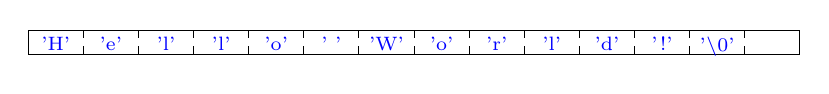
\begin{tikzpicture}[font=\scriptsize,x=1.4cm]
		\draw (0,1) -- (7,1);
		\draw (0,1) -- (0,1.3);
		\draw (0,1.3) -- (7,1.3);
		\draw (7,1) -- (7,1.3);		
		
		\draw[dashed] (.5,1) -- (.5,1.3);
		\draw[dashed] (1,1) -- (1,1.3);
		\draw[dashed] (1.5,1) -- (1.5,1.3);
		\draw[dashed] (2,1) -- (2,1.3);
		\draw[dashed] (2.5,1) -- (2.5,1.3);
		\draw[dashed] (3,1) -- (3,1.3);
		\draw[dashed] (3.5,1) -- (3.5,1.3);
		\draw[dashed] (4,1) -- (4,1.3);
		\draw[dashed] (4.5,1) -- (4.5,1.3);
		\draw[dashed] (5,1) -- (5,1.3);
		\draw[dashed] (5.5,1) -- (5.5,1.3);
		\draw[dashed] (6,1) -- (6,1.3);
		\draw[dashed] (6.5,1) -- (6.5,1.3);
		
		\node[blue, below=-.125em] at (0.25,1.3) {'H'};
		\node[blue, below=-.125em] at (0.75,1.3) {'e'};
		\node[blue, below=-.125em] at (1.25,1.3) {'l'};
		\node[blue, below=-.125em] at (1.75,1.3) {'l'};
		\node[blue, below=-.125em] at (2.25,1.3) {'o'};
		\node[blue, below=-.125em] at (2.75,1.3) {' '};
		\node[blue, below=-.125em] at (3.25,1.3) {'W'};
		\node[blue, below=-.125em] at (3.75,1.3) {'o'};
		\node[blue, below=-.125em] at (4.25,1.3) {'r'};
		\node[blue, below=-.125em] at (4.75,1.3) {'l'};
		\node[blue, below=-.125em] at (5.25,1.3) {'d'};
		\node[blue, below=-.125em] at (5.75,1.3) {'!'};
		\node[blue, below=-.125em] at (6.25,1.3) {'\textbackslash0'};
	\end{tikzpicture}
	\begin{itemize}
		\item Note that '\textbackslash0' is different from the the character '0'
	\end{itemize}
	\ \\\ \\To represent it in an array, you could do the following:
	\begin{lstlisting}[numbers=none]
char hello[] = {'H', 'e', 'l', 'l', 'o', ' ',
				'W', 'o', 'r', 'l', 'd', '!', '\0'};
\end{lstlisting}\ \\
	\ \\But there is a short form for that:
	\begin{lstlisting}[numbers=none]
char hello[] = "Hello World!";
\end{lstlisting}
\end{frame}

\begin{frame}[fragile]{Printing strings}
	You can print strings with printf with the placeholder \textit{\%s}.\\
	It expects an array of chars as an argument:\bigskip
	\begin{lstlisting}[numbers=none]
char hello[] = "Hello World!";
printf("%s\n", hello);
\end{lstlisting}
	\bigskip
	If you don't need any formatting, you can also use \textit{puts}, which has a simpler syntax:
	\begin{lstlisting}[numbers=none]
char hello[] = "Hello World!";
puts(hello);
\end{lstlisting}
\end{frame}

\begin{frame}[fragile]{String input}
	You \textbf{could} use \textit{scanf()} for string input, but it is kind of a mess. You better use \textit{fgets}:
	\begin{lstlisting}[numbers=none]
char input[42];
fgets(input, sizeof input, stdin);
\end{lstlisting}
	\begin{itemize}
		\item \textit{fgets()} reads up to size-1 characters (here: 42-1), and writes the '\textbackslash0' at the end of the array input.
		\item It stops reading after a newline.
		\item \textit{stdin} is the standard input
	\end{itemize}
\end{frame}
\begin{frame}[fragile]{Passing arrays}
	An array is passed by its identifier, no big deal. The real question is, how a function is defined, that takes an array as argument.
	\begin{lstlisting}[numbers=none]
int foo(char arr[]) {
	printf("%d\n", arr[0]);
}
\end{lstlisting}
	\begin{itemize}
		\item \textbf{But:} If you want to get the size of the array in this function, you'll get a false value. The reason for this is discussed later.
		\item Because the size is unknown, you don't know whether an element is safe to access and or already ``out of bounds''
		\item So you may want to pass the size as a second argument
	\end{itemize}
\end{frame}
%
\begin{frame}[fragile]{Arrays of arrays}
	\begin{itemize}
		\item Every sub-array is of the same type
		\item All dimensions apart from the first \underline{must} be specified
		\item Declaration:
		\begin{lstlisting}[numbers=none]
char arr[3][4];
/* an array containing 3 arrays containing 4 chars */
\end{lstlisting}
		\item Assignment:
		\begin{lstlisting}[numbers=none]
arr[0][0] = 'f'; /* first element of arr[0] is 'f' */
arr[1] = "bar";  /* first element of arr is "bar" */
arr[2] = {'b', 'o', 'z', '\0'};
\end{lstlisting}
		\item Definition:
		\begin{lstlisting}[numbers=none]
char arr[][4] = {{'f', 'o', 'o', '\0'},
			     {'b', 'a', 'r', '\0'}};
\end{lstlisting}
	\end{itemize}
\end{frame}
%
\begin{frame}[fragile]{Passing arrays of arrays}
	\begin{itemize}
		\item You can also pass arrays of arrays to functions
		\item Once again, we need to specify the dimensions
		\item Either use fixed values or include dimension arguments in the
		declaration of the array like shown below:
		\begin{lstlisting}[numbers=none]
int foo(char arr[][42]) {
	/* code */
}
int bar(int dim2, char arr[][dim2]) {
	/* code */
}
\end{lstlisting}
	\item The dimension arguments must be passed before the array itself
	\end{itemize}
\end{frame}
% nothing to do from here on
\end{document}
